\appendix
\begin{appendices}

\chapter{Rules of engagement}
\label{app:rules_of_engagement}
\begin{figure}[!h]
	\centering
	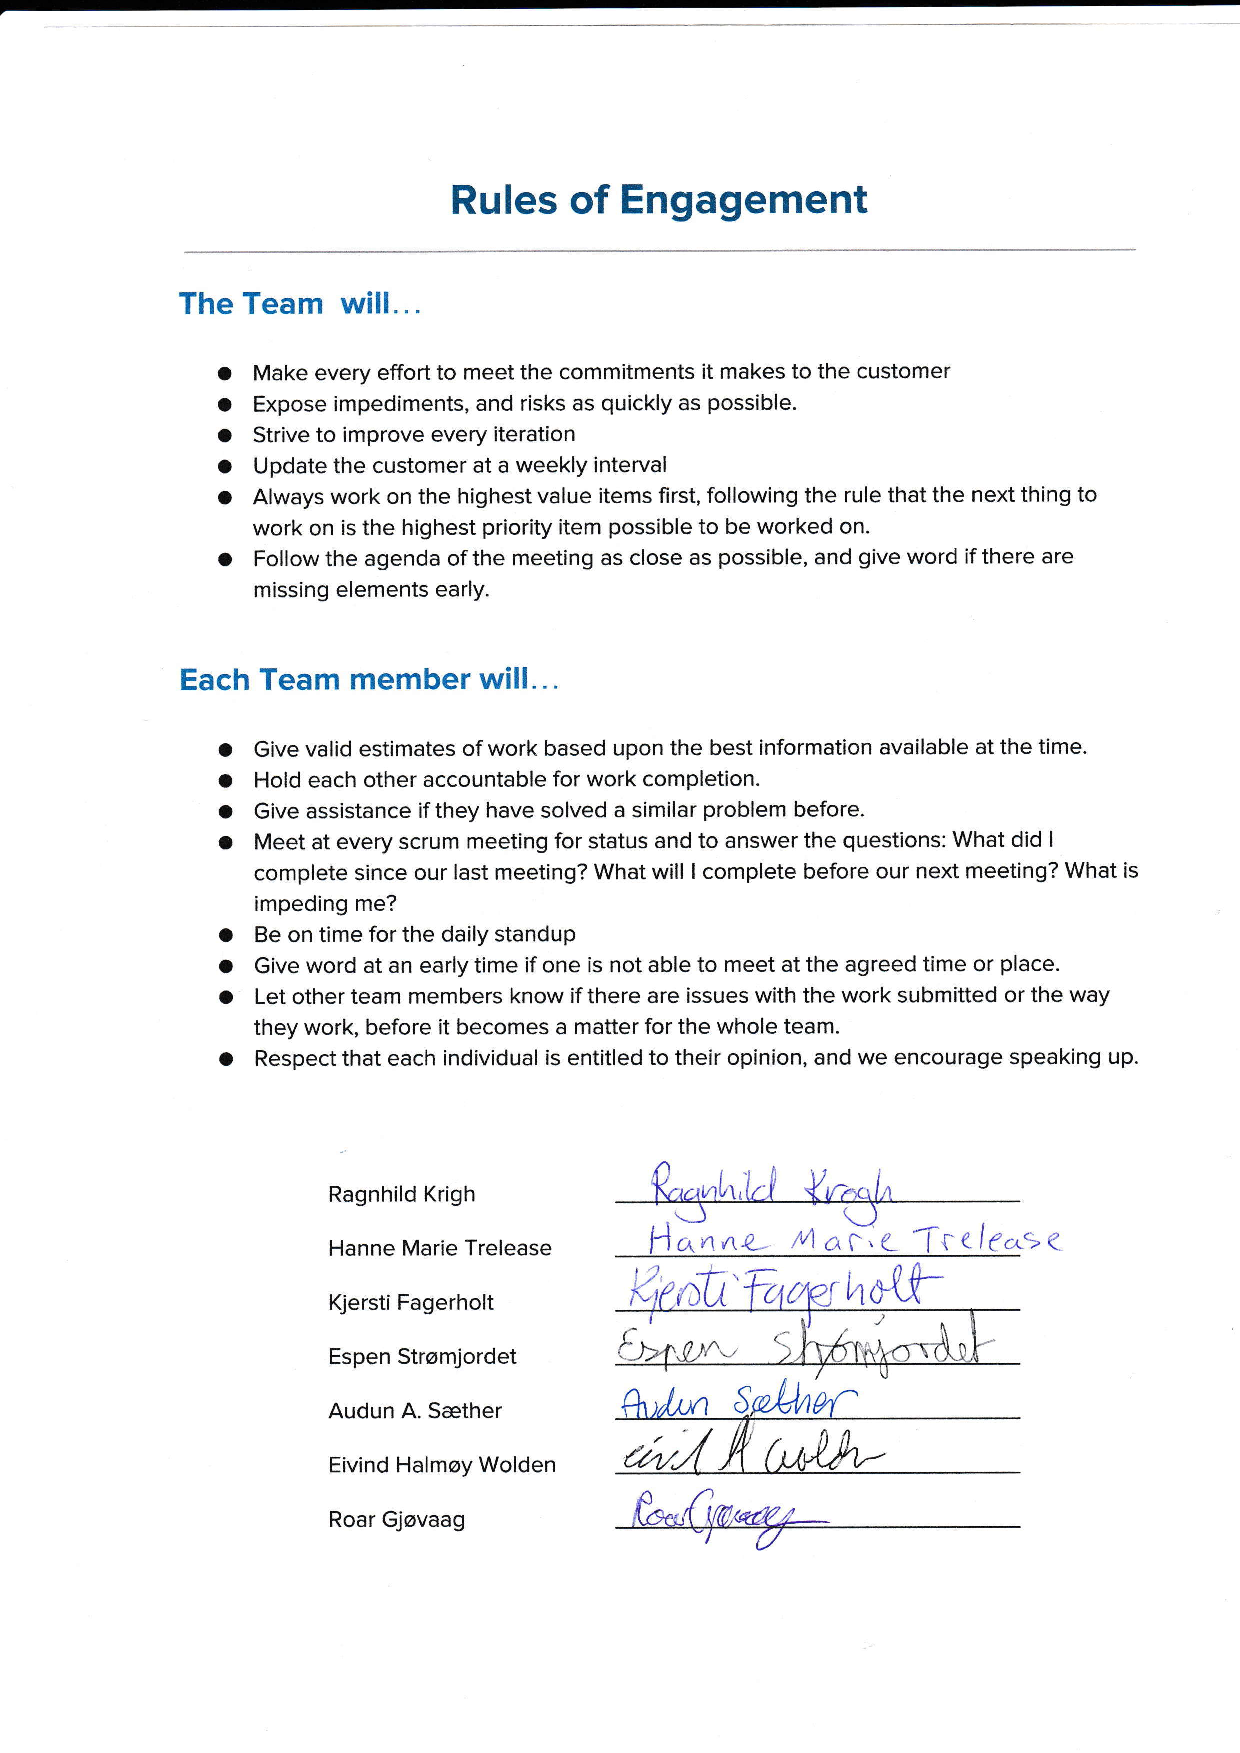
\includegraphics[trim=3cm 3.5cm 1.5cm 3cm,clip,height=13.9cm, width=11cm]{pdffig/RulesOfEngagement}
	\caption{Rules of engagement document}
	\label{fig:rules_of_engagement}
\end{figure}

\chapter{Risk list}
%$\\[0.5cm]$
\label{app:risklist}

L: Likelihood (1-9)\\
I1: Impact (1-9)\\
I2: Importance (Likelihood * Impact)\\
\begin{longtable}{ | p{4.5cm} | p{1cm} | p{1cm} | p{1cm} | p{4.5cm} | p{4.5cm} |}\caption{Risk list}\label{Tab:risklist}\\
	\hline
	\textbf{Description} & \textbf{L} & \textbf{I1} & \textbf{I2} & \textbf{Preventive action} & \textbf{Remedial action} \\ \hline\endhead
	
	
	Underestimate the time planned to use for assignments & 8 & 8 & 64 & Estimate a little higher. continuous meetings. Continuous status update on tasks & Extra work hours and help each other. Have a clear prioritization of tasks so that some less important tasks can be delayed if needed. \\ \hline
	
	The group does not deliver updated information on the report and cannot maximize the quality of the feedback obtained from the supervisor & 6 & 7 & 42 & Always make sure the report meet the demands upon delivery & Ask concrete questions to the supervisor or other competent acquaintances of the group members \\ \hline
	
	An issue in the code that is not understood or can not be fixed. & 5 & 8 & 40 & Comment on the code, and talk with each other about the work done on the code & Get help from the supervisor or other people involved. \\ \hline
	
	The group does not receive quality feedback from supervisor & 6 & 6 & 36 & Be prepared for supervisor meetings. Prepare concrete questions and discuss issues with supervisor & Ask qualified acquaintances to read and give feedback on the report.  \\ \hline
	
	Project complexity / Project too difficult & 5 & 5 & 25 & Do not plan many complicated tasks & Downgrade demands \\ \hline
	
	Poor communication with the customer leading to misunderstandings and doubts about the progress of the project & 4 & 6 & 24 & Be well prepared for meetings by establishing an agenda for the meeting and sharing it with the customer beforehand. Establish a good customer relationship. Send email to the customer for clarification & Send email to the customer for clarification. Cooperate with customer to reprioritize tasks \\ \hline
	
	Poor communication within the group leading to misunderstandings and doubts about the progress of the project & 4 & 6 & 24 & Write meeting minutes to document decisions. Have frequent meetings where every team member explains what they have done and what they are planning to do. & Make a group decision to solve the misunderstanding \\ \hline
	
	Wrong choice of development tools & 4 & 6 & 24 & Do thorough research before deciding which tools to work with & If early in project, consider changing tools \\ \hline
	
	Absence of group member(s) over a period of time & 6 & 4 & 24 & Every member of the group should be aware of what all members are working on, so that they can step in and take over the absent person's tasks & When the progress is halted by a person's absence, other group members should take over the tasks needed for further progress \\ \hline
	
	The workload is distorted. Some members of the group work too much, while others work too little. & 5 & 4 & 20 & Continuous meetings, after every meeting the team members delegate assignments. The leader of the meeting also have to make sure that everyone gets approximately the same amount of work. & Redelegate work tasks within the group. \\ \hline
	
	Poor choice of programming language. It becomes difficult to produce the product before deadline & 2 & 9 & 18 & Good research and discussion in the group. Do not choose a language that some people in the group do not have experience with & Reevaluate non-functional requirements with the customer \\ \hline
	
	Customer changes requirements & 6 & 3 & 18 & Constant communication with customer & Use an agile development process to better adapt to changes \\ \hline
	
	Data loss & 2 & 8 & 16 & Local copy and regular backups & Restore latest available backup \\ \hline
	
	Disagreement within the group on key issues in the project & 3 & 5 & 15 & Establish ground rules regarding how to discuss key issues and how to make decisions final. Make democratic decisions & If the disagreement cannot be solved, one may involve the supervisor \\ \hline
	
	Personal conflicts between group members & 2 & 7 & 14 & Establish ground rules for the team so that emerging conflicts are solved as early as possible & First try to solve the conflict between the group members in question. If this doesn't work, involve the whole group. A last resort would be to involve the supervisor \\ \hline
	
	Product doesn't meet requirements & 2 & 7 & 14 & Request product feedback from customer & Assess which changes must be made and prioritize the most important parts to change \\ \hline
	
	Overestimate the time planned to use for assignments & 3 & 4 & 12 & Investigate the assignments so it is clear what they include, and how much effort it would take to perform them. & When the assignment is done - long before the time, use the extra time on the more time consuming assignments. \\ \hline
	
	Missing deadlines & 1 & 8 & 8 & Have frequent meetings and plan well & Do extra work hours to finish the work as quickly as possible \\ \hline
	
	Product is not user-friendly & 3 & 2 & 6 & Perform usability tests & Assess which changes must be made and prioritize the most important parts to change \\ \hline
	
	Technical issues(server down) & 2 & 3 & 6 & & Use the backup \\ \hline
\end{longtable}

\noindent
\chapter{Requirements}
\label{app:requirements}

\section{Requirements}
\label{app:functional_requirements}

\renewcommand{\arraystretch}{2}
\begin{center}
	\begin{longtable}{ | p{1cm} | p{3cm} | p{5cm} | p{1.5cm} | p{2.5cm} | p{3cm} | }
	\caption[Functional requirements]{The functional requirements listed up and  prioritized by the customers wishes} \\
	
	\hline {\bf ID} & {\bf Name} & {\bf Description} & {\bf Priority} & {\bf Use Case Ref.} & {\bf Comments}\\ \hline
	
		\multicolumn{6}{| >{\columncolor[gray]{0.8}}c |}{General}	\\\hline			
		R1 &  Language & The documentation should be written in english. The application will be written in norwegian and the stories from Digitalt fortalt will appear as they are, most of them in norwegian. & H  &  &  \\\hline
		
		R2& Cross-platform design & The application should run on both Android and iOS. & H &  & 	\\\hline
		
		R3& Cross-platform design & The application design should appear similar on both Android and iOS. & H &  &\\\hline
		\multicolumn{6}{| >{\columncolor[gray]{0.8}} c |}{Sign up /Sign in view}	\\\hline			
		
		R4& User recovery & The application should provide the opportunity for the user to enter email address, which then becomes the user identifier in the system from the user's point of view. & H & U1,U2 & This means that the user can access the profile from different devices.		\\\hline
		
		R5& Anonymous sign in & The application should provide the option to enter the application without registering a user by mail address.  & H & U1 & Device remembers user. User got id in database, but not mail\\\hline
	
		R6& Demo view & It should be possible to run the application mode in a demo view where the system can't identify the user & L &  &				\\\hline
		
		R7& Personal info & The application should obtain some personal info about the user, such as age group and gender. & H & U3 & Only for research purposes \\\hline
		
		\multicolumn{6}{| >{\columncolor[gray]{0.8}} c |}{Preferences/Settings}	\\\hline
		
		R8 & Initial specification of preferences & 
		The user should be asked to set preferences in the startup process. & H & U3 &  \\\hline
		
		R8A & Set category preference & 
		The user should be asked to enter a number of preferred categories. & H & U3 &  \\\hline
		
		R8B & Set location preference & 
		The user should be asked to specify a preferred location. & L & U3 &  \\\hline
		
		R8C & Set notification preferences & 
		The user should be asked to set some preferences about notifications & L & U3 &  \\\hline
		 
		R9&	Changing preferences&  The application should provide a settings view where the user can change the preferences. & H & U9 &	\\\hline
		
		\multicolumn{6}{| >{\columncolor[gray]{0.8}} c |}{Main view: Browse recommended stories}	\\\hline
		
		R10& 
		Show list of recommended stories & The application should provide the user with a list of recommended stories based on the set preferences. The stories is presented by a picture and a short text harvested from Digitalt fortalt. & H & U4  &\\\hline
		R11& Recommend story outside user's preferences  & The application should once in a while recommend a story outside the user comfort zone, i.e. a story that the recommender algorithm does not pick out. & M &  & Purpose: To broaden the user's horizon. The purpose is not to test the algorithm\\\hline		
		
		R12& Make decision about story  & The application should provide the user with three options regarding each recommended story: to choose to read the story now, to reject the story or to save the story for later & H & U4 &\\\hline
		
		\multicolumn{6}{| >{\columncolor[gray]{0.8}} c |}{Story view}	\\\hline
		
		R13& Present story & The application should present the chosen story in a specific story view.The presentation of the story should be in accordance with the presentation on Digitalt fortalt. & H & U6 &\\\hline				
	
		R14& Give feedback/rating on story  & The application should provide the user with the opportunity to rate the story. The rating is in the form of a star system with 5 stars.  & H & U7 &\\\hline
				
		R15 & Tag story / Add story to list  & The user should be given the opportunity to connect a story to tags. The tags could be predefined by the system, like "Les senere" or defined by the user & M  & U5 &\\\hline
		
		R16& Link to Digitalt fortalt  & Every story should include a link to the corresponding story on Digitalt fortalt. & H & U6 &	\\\hline
		
		R17& Explain why a story was recommended & The application should provide an explanation why a given story was recommended. & H & U4 & Could just be a general statement like: "Other users who liked similar stories to you, also liked this one"\\\hline
		
		\multicolumn{6}{| >{\columncolor[gray]{0.8}} c |}{List view}	\\\hline
		
		R18& Show list & The application should show a list of collected stories. The stories is presented by a picture and a short text. & M &  U8 &		\\\hline
		
		R19& Choose list & The application should provide the user with the opportunity to choose different lists. Lists include: to-read,read and user-defined lists & M & U8 &\\\hline
		
		\multicolumn{6}{| >{\columncolor[gray]{0.8}} c |}{Notifications}	\\\hline
		
		R20& Notifications outside the application & The application should send a notification to the user's device at the time specified in the preferences  & L &  &	In agreement with the customer this requirement will not be met			\\\hline
		
		R21& Notifications inside the application & The application should create a notification after a defined amount time to remind the user of stories that have been read but not rated & L &  & In agreement with the customer this requirement will not be met\\\hline
		
		\multicolumn{6}{| >{\columncolor[gray]{0.8}} c |}{About app}	\\\hline
		
		R22 & About the application  & The application should include an about section, which should include basic info about the project. This include references to TAGCLOUD. & H  & U10 &\\\hline
	
		\multicolumn{6}{| >{\columncolor[gray]{0.8}} c |}{Quick tour}	\\\hline
	
		R23A & Quick tour at start up & The application should provide a new user with an explanation of the application at start up.
		& H &  & \\\hline
		
		R23B & Quick tour in menu & The application should provide the opportunity to revisit the quick tour via the menu.
		& L &  & \\\hline
		
		\multicolumn{6}{| >{\columncolor[gray]{0.8}} c |}{Personalization}	\\\hline
		
		R24& Use content-based filtering & The application should use content-based filtering to recommend stories to user initially. This should in particular be based on category preferences. & H  &  & Implement this before R25. \\\hline
		
		R25& Use collaborative filtering & The application should collaborative filtering to recommend stories when the user base is large enough for the algorithm to be effective. & H  &  &\\\hline
		
		\multicolumn{6}{ | >{\columncolor[gray]{0.8}} c |}{Research}	\\\hline		
		
		R26& Gather data to SINTEF for research & The application should gather and store in a file information about the use. This include frequency of use, success rate of recommendations and perhaps other things.  &  &  & Detailed list of what this included provided in mail from the customer. The customer will view this data through the database \\\hline
		
	\end{longtable}
\end{center}
\pagebreak

\section{Quality attributes}
\label{app:quality_attributes}

\begin{table}[!h]
	\centering
	\caption[Quality attributes]{The quality attributes used in this project. Prioritized by the customer} 
	\begin{tabular}{ | p{2.9cm} | p{9.5cm} | p{1.4cm} | p{2cm} | }	
		\hline {\bf Quality \newline attribute} & {\bf Description} & {\bf Priority} & {\bf Optionally; Why?} \\ \hline
			
		Usability & How easy is it for the user to accomplish a desired task and what kind of user support should the system focus on. (eg. tutorials or hints) & 1  & \\\hline
		
		Monitorability & How important is the ability to monitor how the system while its executing. (eg. statistics ect.) & 2 &  \\\hline		
		
		Modifiability & How important and how easy should the product be able to be changed after it`s finalized? (eg. making changes to the UI) & 3 &\\\hline
		
		Performance & How important is time and speed of the system? (eg. response time for fetching stories) & 4 &\\\hline
		
		Interoperability & How important is the ability for the system to work together with other systems. (eg. making use of specific communication protocols or the use of a specified data format) & 5 & 	\\\hline
		
		Availability & How important is the reliability of the product.The easy representation to think of this is uptime of the service. & 6 & \\\hline
	
		Security & How important is the systems ability to protect data and information from unauthorized access. (eg. losing personalized data) & 7 & \\\hline
		
		Testability & How important is the ability to set up tests for the system (eg. setting up automated test for components and parts of the system) & 8 &		\\\hline	
	\end{tabular}
\end{table}

\chapter{Project Management}
\label{app:project_managment} 

\section{WBS Description}
\label{app:wbs_description}


\begin{itemize}
	\item \textbf{Project Management}
	\begin{itemize}
		\item \textbf{Method} \newline
		How does the team work, what kind of development process is used
		\item \textbf{Product Backlog} \newline
		What is to be produced, and estimation of its costs. Maintained on Trello
		\item \textbf{Risk Management} \newline
		What are the project's risks and what is done to counter/prevent them? 
		\item \textbf{Tools} \newline
		What tools are needed to execute the project.
		\item \textbf{Schedule} \newline
		When does the team meet, customer meetings, etc.
		\item \textbf{Rules of Engagement } \newline
		What are the team’s core principles
	\end{itemize}
	\item \textbf{Analysis}
	\begin{itemize}
		\item \textbf{Requirement Specification} \newline
		Specify what the product should be used for
		\begin{itemize}
			\item \textbf{Scenario} \newline
			Describing ways to use the product and in what context
			\item \textbf{Use-Case} \newline
			Describing ways to interact with the product
			
		\end{itemize}
		\item \textbf{Functionalities} \newline
		Define the functionalities of the system
		\item \textbf{Non-Functional Specifications} \newline
		Define the system’s non-functional dependencies	
		\item \textbf{Past Work} \newline
		How does the past work affect this project, what is to be reused and copied	
		\item \textbf{Algorithms} \newline
		What algorithms are of use to the personalization	
		\item \textbf{Framework} \newline
		What framework should be used for the cross-platform development
	\end{itemize}
	\item \textbf{Design}
			\item \textbf{User Interface} \newline
			What should the application look like
			
			\begin{itemize}
				\item \textbf{Concept} \newline
				Making a mockup and iterating
				
				\item \textbf{Prototypes} \newline
				Finalizing the mockup into a prototype to test on customer/users
				
				\item \textbf{IOS} \newline
				What are the distinctions between the systems
				\item \textbf{Android} \newline
				What are the distinctions between the systems
			\end{itemize}
			\item \textbf{System Modeling} \newline
			Top-level software design
			
			\begin{itemize}
				\item \textbf{Architecture} \newline
				How is the system built, how does the component fit together
				\item \textbf{Documentation} \newline
				Detailed software design
				
			\end{itemize}
			\item \textbf{Database Modeling} \newline
			Model how the database should work
			\begin{itemize}
				\item \textbf{Documentation} \newline
				Detailed database design
			\end{itemize}
	\item \textbf{Development}
			\item \textbf{Back-end} \newline
			\begin{itemize}
				\item \textbf{Database} \newline
				Implementing a database
				\item \textbf{Harvesting} \newline
				Harvest the data from Digital Fortalt
				
				\item \textbf{Personalizing } \newline
				Main objective for the project
				\begin{itemize}
					\item \textbf{Collaborative Filtering} \newline
					Filter content on the basis of other users
					\item \textbf{Content-based Filtering} \newline
					Filter content on the basis of you past feedback
				\end{itemize}
				\item \textbf{Server} \newline
				Getting the server up and running managing reboots and updates
				\item \textbf{Front-end Communication} \newline
				How should the system communicate with front-end
				\item \textbf{Research Data} \newline
				I what way would the research data be recorded and saved
				\item \textbf{Feedback} \newline
				Handling feedback
				\begin{itemize}
					\item \textbf{Bug-fixing} \newline
					Setting a side time for fixing bugs
					\item \textbf{Customer Adjustment} \newline
					Be ready for requirement modifications and small adjustments on functionalities
				\end{itemize}
			\end{itemize}
			\item \textbf{Front-End} \newline
			\begin{itemize}
				\item \textbf{IOS / Android} \newline
				\begin{itemize}
					\item \textbf{Onboarding} \newline
					Make a introduction for the application
					\item \textbf{List} \newline
					Make stories viewable in a list 
					\item \textbf{Login} \newline
					Login view
					\item \textbf{Story} \newline
					Presenting a story in accordance with the source
					\item \textbf{Recommendation } \newline
					View to present the recommendations 
					\item \textbf{Settings} \newline
					View for changing the personal settings
				\end{itemize}
				\item \textbf{Research Data} \newline
				Log and send the research data
				\item \textbf{Feedback} \newline
				Accommodate user feedback and customer feedback 
				\begin{itemize}
					\item \textbf{Bug-fixing} \newline
					Setting a side time for fixing bugs
					\item \textbf{Customer Adjustment} \newline
					requirement modifications and UI adjustments.
				\end{itemize}
				\item \textbf{Back-end Communication} \newline
				Set up communication with back-end
			\end{itemize}
	\item \textbf{Testing}
		\begin{itemize}
			\item \textbf{Unit Testing} \newline
			Complete unit test on as many function as feasible 
			\item \textbf{Component Testing} \newline
			Complete component testing on relevant modules and components 
			\item \textbf{Integration testing} \newline
			Test the integration between the modules
			\item \textbf{System testing} \newline
			Test the system as a whole
			\item \textbf{User Testing } \newline
			Test the application on potential users 
			\item \textbf{Acceptance testing} \newline
			Preform a acceptance test on the customer 
		\end{itemize}
	\item \textbf{Documentation}
		\begin{itemize}
			\item \textbf{Theory} \newline
			Find relevant theory for the project 
			\item \textbf{Commenting} \newline
			Well commented code 
			\item \textbf{Justification} \newline
			Justify decisions 
			\item \textbf{Logging} \newline
			Log meeting, activities and work hours
			\item \textbf{Licensing} \newline
			Update and write about the licensing deal, on repositories and other relevant places 
		\end{itemize}
\end{itemize}


\chapter{Status report example}
\label{app:status_report}

\todo{Tror ikke det er referert til status-rapportene noe sted i hoveddelen av rapporten}
Status report week 6\newline


		\textbf{Introduction} \newline
		This week has mostly been spent organising and making decisions that will impact the whole project.\newline
		
		\textbf{Progress summary} \newline
		The decisions that have been made will decide how the work is distributed in the coming weeks. Work has been made on defining goals and milestones. Furthermore, some of the tools to complete the given tasks have been found.\newline
		
		\textbf{Open / closed problems}\newline
		Closed problems:
		\begin{itemize}
			\item A cross-platform framework have been chosen.
			\item A rough estimate of what needs doing, how long it will take and when it is due has been performed in the form of a product backlog.
			\item A list of functional requirements have been compiled after a discussion with the customer.
			Use case diagrams and scenarios have been made.
			\item Justification on some of the choices made so far have been written for the report:
			\begin{itemize}
				\item Scrum
				\item Framework
			\end{itemize}
			\item Complete a WBS chart.
			\item A rules of engagement have been signed, this helps solidify what is expected of every member in the group.\newline
		\end{itemize}
		
		Open problems:\newline
		No specific ongoing problem at the end of this week.\newline
		
		Choosing a cross-platform framework was a difficult process for various reasons. There is not much experience in the group using such tools. Additionally there was an internal debate about what is expected from the customer and what does the team expect the end product to look like. This was discussed in light of the the constraints imposed from various aspects. However, the team members now feel confident that an appropriate tool have been chosen and are aware of some limitations this leads to.\newline
		
		Understanding properly what the customer wants and prioritizes has also been a focus this week. While this sounds easy enough, the technical details are often lost in communication. This is something that will require constant feedback and monitoring so that the project stays on track in regards to what is desired by the customer.\newline
		
		\textbf{Planned work for next period}\newline
		\begin{itemize}
			\item Familiarization with the chosen framework.
			\item Familiarization with digitaltfortalt.no API.
			\item Creating a design prototype is a goal, this will unify the group and make sure all members are working towards the same goal. Furthermore, this will explore what options there are and highlight any basic flaws in design.
		\end{itemize}
\raggedbottom
\newpage		

\chapter{Unit test cases}
\label{app:unittest}
\renewcommand{\arraystretch}{2}%
\begin{center}
	\begin{longtable}{ | p{1cm} | p{5.5cm} | p{4cm} | p{4.5cm} | p{2cm}|}
		\caption[Unit Test cases]{ Here presented by a testId, description of how the test should be perfomed, what input data to use and expected results.} \label{Tab:unittestcases}\\
		
		\hline {\bf Test case ID} & {\bf Description} & {\bf Input data} & {\bf Expected results} & {\bf Result}\\ \hline
		
		\multicolumn{5}{| >{\columncolor[gray]{0.8}} c |}{Unit 1: Database Helper}	\\\hline
		
		
		UN1.1 & Update one rating value in the database & Random userId, random storyId, updateValue: 2 & The function should return true when running the database request. & Pass \\\hline
		
		UN1.2 & Update rating values in the database & Random userId, random storyId, update Value : 5 & The function should return true when running the database request & Pass\\\hline
		
		UN1.3 & Update new tag that user have created & Random userId, tagName: 'NyTestTag2' & The function should return true when running the database request& Pass \\\hline
		
		UN1.4 & Update a users tag which is connected to a story & Random userId, Random storyId, tagName: 'Les senere' & The function should return true when running the database request& Pass \\\hline
		
		UN1.5 & Update a users action of rejecting a story & Random userId, Random storyId & The function should return true when running the database request & Pass \\\hline
		
		UN1.6 & Update a story as recommended & Random userId, Random storyId & The function should return true when running the database request & Pass\\\hline
		
		UN1.7 & Get rating on a story done by a user  & Random userId, Random storyId & Should return row with the rating presented as a integer & Pass\\ \hline			
		
		UN1.8 & Get the predefined tags connected to a user & Random userId & Should return row with the tags "Les senere" and "Les" which all users in the system is connected to. If this user has self made tags, they should be included & Pass\\ \hline
		
		UN1.9 & Get all the tags connected to a user & Specified userId: 105 & Should return row with the tags "Les senere" and "Les" which all users in the system is connected to, included the added tag 'NyTestTag' & Pass\\ \hline
		
		UN1.10 & Get the tags connected to a story and a user & Specified userId: 105, specified storyId: 'DF.1295' & Should return row with the tag 'NyTestTag' & Pass \\ \hline
		
		UN1.11 & Get stories with timestamp & -  & Should return rows with 167 storyId and a timestamp which indicate when the story was last changed & Pass \\ \hline
		
		UN1.12 & Get subcategories to a specific story & Random storyId & Should return a row with an array of subcategory Ids & Pass\\ \hline
		
		UN1.13 & Get story information & Specified userId: 105, specified storyId: 'DF.5220' & Should return row with an array with the keys: userId, storyId, explanation, rating, false\textunderscore recommend, recommended\textunderscore ranking, in\textunderscore frontend\textunderscore array, estimated\textunderscore Rating & Pass  \\ \hline
		\multicolumn{5}{| >{\columncolor[gray]{0.8}} c |}{Unit 2: Database Story}	\\\hline			
		
		UN2.1 & Fetch Story & Specified storyId: 'DF.1812', specified userId: 105 & Should return row with an array of the categories to the story and tags and tagName that are connected to the userId  & Pass\\ \hline
		
		UN2.2 & Get recommended stories for a user & random userId &  Should return 10 rows with stories, and they should include: userId, storyId, recommended\textunderscore ranking, explanation, false\textunderscore recommend, title, introduction, author, categories and mediaId & Pass\\ \hline
		
		UN2.3 & Get list of stories which is tagged by a user & Specified userId: 103, tagName: 'NyTestTag' & Should return rows with stories, and they should include: storyId, title, author, introduction, date, tagName, categories and mediaId & Pass\\ \hline
		
		UN2.4 & Get subcategories per story & - & Should return 167 stories  with numericalId and subcategory ids  & Pass\\ \hline
		
		UN2.5 & Get all stories with storyId, numericalId and categories & - & Should return 167 rows with storyId, numericalId and categories & Pass\\ \hline
		
		UN2.6 & Get states per story  & Specified userId: 258, specified storyId: 'DF.1600'& Should return a row with stateId, numTimesRecorded and latestStateTime &  Pass\\ \hline
		\multicolumn{5}{| >{\columncolor[gray]{0.8}} c |}{Unit 3: Database User}	\\\hline
		
		
		UN3.1 & Add user   & example mail: example@example.com & Should return a userId that is not null &  Pass\\ \hline
		
		UN3.2 & Get user from Id & UserId: generated new Id. & Should return a userId from the database which is equal the userId input & Pass\\ \hline
		
		UN3.3 & Update user mail &UserId: generated new id,\newline email: newmail@example.com &  Should return a email from the database which is equal the email input & Pass\\ \hline
		
		UN3.4 & Update user age & UserId: generated new Id ,\newline age group: 0 & Should return a user model from the database, which includes the age group that is equal to the age group input.  & Pass\\ \hline
		
		UN3.5 & Update user categories & UserId: generated new id, \newline category preference: [2] & Should return a row with user model from the database with the category preference that is equal to the category preference input.  & Pass\\ \hline
		
		UN3.6 & Get user from email & UserId: generated new id, \newline email:54@example.com & Should return a user model from the database, which includes the mail that is equal to the email input.   & Pass\\ \hline							
		
		UN3.7 & Get user categories & UserId: generated new id, \newline category preferences: [1,3,5,7,9] & Should return the categories from the database that is equal to the category preferences input  & Pass\\ \hline
		
		UN3.8 & Get user mail from Id  & UserId: generated new id  &  Should return a  user model from the database,which includes the email that is equal the email input. & Pass\\ \hline
	
		\multicolumn{5}{| >{\columncolor[gray]{0.8}} c |}{Unit 4: User Model}	\\\hline
		
		UN4.1 & Initiate User   & userId:1, \newline mail: example@example.com & Should create a user model with the correct input. The getters should return the values that matches with the input values& Pass\\ \hline
		
		UN4.2 & Set all user details &userId:1, \newline mail: example@example.com,gender: 0, age group: 1, use of loc. : 0 , category preference: [1,3,5,7,9] & Should add the correct user details to the user model. The getters should return the values that matches with the input values  & Pass\\ \hline
		
		UN4.2 & Print All  &  userId:1, \newline mail: example@example.com,gender: 0, age group: 1, use of loc. : 0 , category preference: [1,3,5,7,9] & The printAll function should return a string with all the correct attributes and values that matches the input values .   & Pass\\ \hline
		
		\multicolumn{5}{| >{\columncolor[gray]{0.8}} c |}{Unit 5: Compute Preference Value}	\\\hline
		
		
		UN5.1 & Compute preference value for all stories for a  user & Random userId & Should return 167 rows from the database, and every row should include: storyId, userId, numericalId and preferenceValue  & Pass\\ \hline
		
		UN5.2 & Compute preference value of a story for a user  & Random userId , specific 'DF.1098' & Should return an array with userId, storyId, numericalId and the preference value& Pass\\ \hline
		
		UN5.3 & Compute preference value & Specific storyId  & Should return the preference value which is the type double & Pass\\ \hline
		\multicolumn{5}{| >{\columncolor[gray]{0.8}} c |}{Unit 5: Run Recommender}	\\\hline
		
		
		
		
		\multicolumn{5}{| >{\columncolor[gray]{0.8}} c |}{Unit 6: Recommendation}	\\\hline
		
		UN6.1 & Run recommender & Random userId  & & Pass\\ \hline	
		
		UN6.2 & New content based recommendation & Input: setUp.xml - a data model with userIds and connected preference values. & The recommender should return the correct number of recommendations when it should create new ones &  Pass\\ \hline			
		
		UN6.3 & Add content based recommendation & Input: setUp.xml- a data model with userIds and connected preference values. & The recommender should return the correct number of recommendations when its adding recommendations to existing ones & Pass\\ \hline	
		
		\multicolumn{5}{| >{\columncolor[gray]{0.8}} c |}{Unit 7:  Database connection with Java}	\\\hline
		
		UN7.1 & Insert recommendation  & userId: 1,\newline  storyId: Df.1098,\newline DF.1501,\newline explanation: 0, \newline false\textunderscore rec. :0, \newline ranking: 3,4,\newline estimatedValue: 0,0 & Expected table in XML-representation(insert-expected.xml) is the same as the actual from the database & Pass\\ \hline			
		
		UN7.2 & Insert Update  & userId: 1, \newline storyIds: DF.1709,DF.1849, \newline explanation:“updated”, \newline false\textunderscore rec. : 1,0, \newline typeoffrec. :1,1, \newline  ranking: 3,4 estimatedValue: 4.5, 2.5   & Expected table in XML-representation(insertUpdate-expected.xml) is the same as the actual from the databas & Pass\\ \hline										
		
		UN7.3 & Delete recommendations & UserId: 1 & Expected table in XML representation(delete-expected.xml)  is the same table returned from DB & Pass\\ \hline		
		
		UN7.4 & Rated  & UserIds: 3,5 \newline	numericalId: 1812,1901 & The getRated function should fetch the correct stories. The input rating should be the same as the returned ratings & Pass \\ \hline						
		UN7.5 & Test frontend array & Numerical Ids: 1849, 1901  & Get stories from frontend array should match the fronted array in XML format(setUp.xml) & Pass\\ \hline	
		
		UN7.6 & Create explanation  & Numerical Ids: 1098,1115,1501  & The create explanation function should return a string with the correct storyIds and their titles. & Pass\\ \hline								
		
		\multicolumn{5}{| >{\columncolor[gray]{0.8}} c |}{Unit 8: UI-Log in}	\\\hline			
		
		UN8.1 & Log in with an already existing user\newline - Check if response is correct & existinguser@\newline mail.no & The user should get access and be directed to the recommendation view(main view) & Pass \\ \hline			
		
		UN8.2 & Log in with a non-existing user \newline - Check if response is correct & “newemail@\newline gmail.com” & The user should get access and be directed to the setup view.& Pass \\\hline	
		
		UN8.3 &  Login a user with the wrong email format \newline - Check if response message is correct & “newemail” & The user should not get access and get a textual response from the system that the format of the input is wrong.& Pass\\ \hline	
		
		\multicolumn{5}{| >{\columncolor[gray]{0.8}} c |}{Unit 9: UI-Story View}	\\\hline			
		
		UN9.1 & If story contains sound clip or video, check if these are presented properly & - story with video\newline
		-story with sound clip & Should show the presence sound clip and video in the tabs. Should be able to handle the different video types, and be able to play them. & Pass \\ \hline			
		
		UN9.2 & Give a rating\newline - Check if the stars change color and response message are visible to the user.  & & Stars should change color when user performs rating, and the user should get a response message from the system which says that this story has been rated. & Pass \\\hline	
		
		UN9.3 & Give the story a new bookmark with a name\newline -add this \newline -Check if response message is visible to the user  & “new bookmark”  & When a new bookmark is made and the story is stored here, the user should get response message about this.& Pass\\ \hline	
		
		\multicolumn{5}{| >{\columncolor[gray]{0.8}} c |}{Unit 10: Settings}	\\\hline					
		
		UN10.1 & Update profile with the wrong email format  & updateemail  & The user should get a response message from the system that the input was not valid and that the user should try again. & Pass  \\ \hline
		
		UN10.2 & Update profile with a email that already exists in the system  & “alreadyexistingemail\newline @email.com”  & The user should get a response message from the system that the input was not valid and that the user should try again.   & Pass \\\hline	
		
		
	\end{longtable}
\end{center}
\raggedbottom
\newpage		


\chapter{Integration test cases}
\label{app:integrationtest}
\renewcommand{\arraystretch}{2}%
\begin{center}
	\begin{longtable}{ | p{1cm} | p{5.5cm} | p{4cm} | p{4.5cm} | p{2cm}|}
		
		\caption[Integration Test Cases]{Integration Test Cases} \label{Tab:integrationtestcases}\\
		\hline
		\textbf{Test case ID} & \textbf{Description} & \textbf{Input data} & \textbf{Expected results} & \textbf{Result} \\ \hline
		
		I.1 & Simulate a HTTP request which will log in a user for the first time with an email adress \newline Call getUserFromEmail to the database & email: 'testnr16@example.com,\newline requestType: addUser & The HTTP request should return successfull message included the newly created userId. The database  function should return a row with the userId, mail, age\textunderscore group, gender and use\textunderscore of\textunderscore location  & Pass \\ \hline
		
		I.2 & Simulate a HTTP request which will log in a user for the first time without an email adress. /newline Call getUserFromId to the database & email:null, \newline request type:addUser  & The HTTP request should return a successful message included the newly created userId The database function should return the usermodel containing userId, mail, age\textunderscore group, gender and user\textunderscore of\textunderscore location.  & Pass \\ \hline
		
		I.3 & Simulate a HTTP request which will update a users profile. \newline Call getUserFromId to the database.  \newline Check if the updates where correct & email: 'testMail23@example.com', request type: updateUser,  & The HTTP request should return a successfull message. The database function should return a usermodel where the email match the input.& Pass\\ \hline
		
		I.4 & Simulate a HTTP request that will create a new test user without an email, Simulate another HTTP request which will update email to this test user, with an email that already exists in the system \newline  Call the getUserFromId function to the database. \newline Check if the user is not updated & email: 'testMail23@example.com' & The HTTP request should return a failure message. The database function should return an usermodel where the email is null. & Pass\\ \hline
		
		I.5 & Simulate a HTTP request that will create a new test user without an email, \newline Simulate another HTTP request which will update email to this test user \newline  Call the getUserFromId function to the database. \newline Check if the user is updated &  & The HTTP request should return a successfull message. The database function should return an usermodel where the email matches the input. & Pass\\ \hline
		
		I.6 & Simulate a HTTP request that will create a new test user with an email\newline  Simulate another HTTP request that will return the user model from the users email \newline Check if the returned data has all attributes required, and that the data match with the input data & email: 'getUserFromEmailTest@example.com",\newline request type: addUser/getUserFromEmail  & The HTTP request should return a usermodel with the attributes userId, email, age\textunderscore group, gender, use\textunderscore of\textunderscore location and with the data which match the input data.& Pass \\ \hline
		
		I.7 & Simulate a HTTP request that will create a new test user without an email\newline  Simulate another HTTP request that will return the user model from the users id \newline Check if the returned data has all attributes required, and that the data match with the input data & email: null,\newline request type: addUser/getUserFromId  & The HTTP request should return a usermodel with the attributes userId, email, age\textunderscore group, gender, use\textunderscore of\textunderscore location and with the data which match the input data. & Pass\\ \hline
		
		I.8 & Simulate a HTTP request that will create a new test user without an email. \newline Call the getNumberOfRatingsDoneByThisUser to the database \newline  Simulate another HTTP request which will connect a rating to a story for this user.  \newline Call the getNumberOfRatingsDoneByThisUser to the database again \newline Check if another rating is registered & email: null,\newline request type: rating, storyId: 'DF.52201, random userId  & The HTTP request should return a usermodel with the attributes userId, email, age\textunderscore group, gender, use\textunderscore of\textunderscore location and with the data which match the input data. & Pass \\ \hline
		
		%THIS IS NOT DONE YET
		I.9 & Simulate a HTTP request that will create a new test user without an email. \newline  \newline  Simulate another HTTP request where the user rejects a story.  \newline  \newline Check if the rejection is stored & email: null,\newline request type: rejectStory  &  & Pass \\ \hline
		
		I.10 & Simulate a HTTP request that will create a new test user without an email. \newline  Simulate a  request that will create a new tag for this user \newline Simulate a HTTP request that will return the list of tags for this user \newline Check if the new tag has been added  & request type: addUser/addNewTag/getList  tagName: 'newTag1' & The returned list should only include the one tag that where created.& Pass\\ \hline
		
		I.11 & Simulate a HTTP request that will create a new test user without an email. \newline  Simulate a HTTP request that will create a new tag for this user \newline Simulate a HTTP request that will return the list of stories contained in this taglist \newline Check if the new tag has been added  & request type: addUser,tagStory,getList \newline tagName: 'newTag1',\newline storyId: 'DF.5223' & The returned list should have the recently added story in the top of the list. The list should have the following attributes connected to every story: id, title, description, false\textunderscore recommend, explanation, picture, thumbnail, categories, mediaType, author, data  & Pass\\ \hline
		
		I.11 & Simulate a HTTP request that will create a new tag for a user. \newline  Simulate a HTTP request that will return all the tags connected to this user \newline Check if the tag was stored \newline Simulate a HTTP request that will remove the new tag that were created earlier \newline Simulate another HTTP request that will return all the tags connected to this user \newline Check if the new tag has been removed  & Specified userId: 105, \newline request type: addnewTag, getAllLists, removeTag,\newline tagName: 'tagToBeRemoved',\newline storyId: 'DF.6081' & The returned list should have the recently added story in the top of the list. The list should have the following attributes connected to every story: id, title, description, false\textunderscore recommend, explanation, picture, thumbnail, categories, mediaType, author, data  & Pass\\ \hline
		
		
		I.12 & Simulate a HTTP request that will return the list connected to a tag for an user  & Specified userId: 105, request type: getList,\newline tagName: 'Les senere' & Should return a list of the stories connected to this tag. The stories should have the following attributes: id, title, description, false\textunderscore recommend, explanation, picture, thumbnail, categories, mediaType, author, date & Pass\\ \hline					
		
		
		I.13 & Simulate a HTTP request that will return all the tags connected to a user  & Specified userId: 105, \newline request type: getList, \newline tagName: 'Les senere' & Should return a list of the tags. The tags should have the attributes text and checked. & Pass\\ \hline	
		
	\end{longtable}
\end{center}
\raggedbottom
\newpage		

\chapter{System test cases}
\label{app:systemtest}

\begin{table}[H]
	\centering
	\caption{System test case for creating a recoverable profile.}
	\begin{tabular}[b]{ | l | l  |}
			\hline
			\textbf{Test ID} & T1  \\ \hline
			\textbf{Test Item} & Create recoverable profile \\ \hline
			\textbf{Approach} & \begin{minipage}{5in}The user locate and press the “register user” button in the app. Applies the email in the correct format.. The response is valid and the user gets feedback. \end{minipage}\\ \hline
			\textbf{Input data} &  “newuser@example.com”\\ \hline
			
			\textbf{Expected results} & \begin{minipage}{5in}The user writes the correct email address and get the correct feedback from the system: "Kontakter server" and will be directed to the startup page.\end{minipage}\\ \hline&\\[-3.8ex]
		
			\textbf{Testing task} & \begin{minipage}{5in}
			\begin{enumerate}[noitemsep]
			\item Click  “create user”-button.
			\item Apply email address to the email input field 
			\item Receive feedback feedback from the system
			\item Check email inbox to se if the correct mail from the system was received 
			 \end{enumerate} \end{minipage}
			\\&\\[-3.8ex] \hline
			\textbf{Depends on tests}& NaN \\ \hline	
			\textbf{Pass/Fail} & Passed \\\hline				
		\end{tabular}
	\label{Tab:systemTesting1}
\end{table}


	\begin{table}[H]
		\centering
		\caption{System test case for login with email registration}
		\begin{tabular}{ | l | l  |}
			\hline
			\textbf{Test ID} & T2  \\ \hline 
			\textbf{Test Item} & Log in with email registration \\ \hline
			\textbf{Approach} & \begin{minipage}{5in}The user locate the login-button and applies the registrated email and obtain access to the system and the profile connected to this email address . \end{minipage}\\ \hline
			\textbf{Input data} &  valid email: “user@example.com”, \newline example invalid email: “mail@example”\\ \hline&\\[-3.8ex]
			\textbf{Expected results} & \begin{minipage}{5in}
			\begin{itemize}[noitemsep]
				\item The first time the user have logged in \newline System Response:  Choose preferences-view should appear.
				\item The user have done this process before \newline System Response: "Vennligst vent mens vi finner historier vi tror du vil like" and direct the user to the view with the recommended stories.
				\item The user types an email with wrong email format \newline System Response: "Ikke en gyldig adresse" 
				
			\end{itemize} \end{minipage}
			 \\ &\\[-3.8ex]\hline&\\[-3.8ex]
			\textbf{Testing task} & \begin{minipage}{5in}
			\begin{enumerate}[noitemsep]
			\item Navigate to the login view
			\item Apply email address to the email input field
			\item Receive response from system
			\end{enumerate}\end{minipage}
			 \\ &\\[-3.8ex]\hline
			\textbf{Depends on tests} & T1 \\ \hline					
			\textbf{Pass/Fail} & Passed \\\hline
		\end{tabular}
	
	\label{Tab_systemTesting2}
	\end{table}

	\begin{table}[H]
		\centering
		\caption{System test case for initial settings}
		\begin{tabular}{ | l | l |}			
			\hline
			\textbf{Test ID} & T3  \\ \hline
			\textbf{Test Item} & Set initial settings \\ \hline
			\textbf{Approach} & \begin{minipage}{5in}The user is logged in to the system for the first time. The user will choose age group and gender in the inital settings that will appear the frist time the user is logged on to the system. After this the user will be asked to choose cultural category preferences.  \end{minipage}\\ \hline
			\textbf{Item pass/Fail criteria} & \\ \hline
			\textbf{Input data} & \begin{minipage}{5in} User action: click the buttons for the age group, gender and interests, and next buttons  \end{minipage}\\ \hline
			\textbf{Expected results} & \begin{minipage}{5in}The user will click the buttons for age group, gender, and interests. The buttons will change color when clicked on. The user navigates to next view by clicking the next button and will obtain access to the system. If the user do not select interests the user will get a response for the system that it is necessary. \end{minipage}\\ \hline&\\[-3.8ex]
			\textbf{Testing task} & \begin{minipage}{5in}
			\begin{enumerate}[noitemsep]
				\item Start app
				\item Click the correct age group and gender.
				\item Navigate to the next page
				\item Navigate to the next page without selecting interests
				\item Receive feedback from system
				\item Select two interests
				\item Navigate to the next page
			\end{enumerate}\end{minipage}
			\\ &\\[-3.8ex]\hline
			\textbf{Depends on tests} & NaN \\ \hline	
			\textbf{Pass/Fail} & Passed \\\hline				
		\end{tabular}
	\label{Tab:systemTesting3}
	\end{table}


	\begin{table}[H]
		\centering
		\caption{System test case for browsing recommended stories}
		\begin{tabular}{ | l | l  |}
			\hline
			\hline
			\textbf{Test ID} & T4  \\ \hline
			\textbf{Test Item} & Browse recommended stories \\ \hline
			\textbf{Approach} & \begin{minipage}{5in}The user is shown a list of recommended stories. The user will click on the first story. The story will be viewed and the user closes it. 
			\end{minipage}\\ \hline
			\textbf{Item pass/Fail criteria} &  \\ \hline			
			\textbf{Input data} &  User action: click arrow\\ \hline
			\textbf{Expected results} & \begin{minipage}{5in}The view should show a list with recommended stories. The view of the stories will include a title, story picture or default picture, an introduction, category icons, media icons and a explanation of why this story is recommended to the user.  The view should show 10 more recommendations when the user have browes through the 10 first stories in the list.
			When the user clicks a story the full story should appear in a full screen, including text and potential pictures, videos and sound clips.   \end{minipage}\\ \hline&\\[-3.8ex]
			\textbf{Testing task} & \begin{minipage}{5in}
			\begin{enumerate}[noitemsep]
			\item Click on a recommended story
			\item Locate back-button and close the story
			\item Click on the next recommended story
			\item Navigate 
			\end{enumerate}\end{minipage}
			\\ &\\[-3.8ex]\hline
			\textbf{Depends on tests} & T1,T2 \\ \hline		
			\textbf{Pass/Fail} & Passed \\\hline			
		\end{tabular}
	
	\label{Tab:systemTesting4}
	\end{table}


	\begin{table}[H]
		\centering
		\caption{System test case for adding a story to list}
		\begin{tabular}{ | l | l  |}
			\hline 
			\textbf{Test ID} & T5  \\ \hline
			\textbf{Test Item}  & Add story to list	 \\ \hline
			\textbf{Approach} & \begin{minipage}{5in}The user navigate to a story and gives the story a rating. The user clicks the bookmark button in the story, and gives a name to a new list of stories.   \end{minipage}\\ \hline
			\textbf{Input data} & \begin{minipage}{5in}User action: Click on a star, Give name to a new list of stories: ex. “My Favorite Stories” \end{minipage}\\ \hline
			\textbf{Expected results} & \begin{minipage}{5in}The story that was rated with stars are automatically put in the “read” list. The story should be stored in the new list of “My Favorite Stories” and the user have access to this by navigating to the menu, and then to “Bokmerker”. \end{minipage}\\ \hline&\\[-3.8ex]
			\textbf{Testing task} & \begin{minipage}{5in}
			\begin{enumerate}[noitemsep]
			\item Click on a story in the recommendation view 
			\item Click on the star icon to in the right upper corner 
			\item Click on one of the stars in the rating view to give rate.
			\item Click out from the view. 
			\item Click the bookmark button in the story 
			\item Click the plus icon
			\item Type in a "My Favorite Stories" and click out of the view.
			\item Navigate to the lists via the menu
			\item Click on "My Favorite Stories"
			\item Click on the first story in the list
			\item Navigates to the “read” list
			\item Click on the first story in the list
			\end{enumerate}\end{minipage}
			\\ &\\[-3.8ex]\hline
			\textbf{Depends on tests} & NaN \\ \hline			
			\textbf{Pass/Fail} & Passed \\\hline		
		\end{tabular}
	
	\label{Tab:systemTesting5}
	\end{table}
	


	\begin{table}[H]
		\centering
		\caption{System test case for giving rating}
		\begin{tabular}{ | l | l  |}
			\hline
			\textbf{Test ID} & T6  \\ \hline
			\textbf{Test Item} & Give a rating \\ \hline
			\textbf{Approach} & \begin{minipage}{5in}The user gives a story a rating by clicking the stars. The user navigates to bookmark lists and checks if the story was stored in the “read” list \end{minipage}\\ \hline
			\textbf{Input data} &  \begin{minipage}{5in}User action: clicks on story, navigated to rating view, clicks on a star. \end{minipage}\\ \hline
			\textbf{Expected results} & \begin{minipage}{5in}The star buttons that were pressed will change color.  The system should store the rating for that story. The next time the user clicks on this story - the yellow stars will show the users rating.  \end{minipage}\\ \hline&\\[-3.8ex]
			\textbf{Testing task} & \begin{minipage}{5in}
			\begin{enumerate}[noitemsep]
			\item Click on a story in the recommendation view
			\item Click on the star icon to in the right upper corner
			\item Click on one of the stars in the rating view to give rate.
			\item Click out from the view. 
			\item Click on the star icon again
			\item Close rating view
			\end{enumerate}\end{minipage}
			\\ &\\[-3.8ex]\hline
			\textbf{Depends on tests} & T1,T2 \\ \hline		
			\textbf{Pass/Fail} & Passed \\\hline			
		\end{tabular}
	\label{Tab_systemTesting6}
	\end{table}




	\begin{table}[H]
		\centering
		\caption{System test case for specifying settings}
		\begin{tabular}{ | l | l  |}
			\hline
			\textbf{Test ID} & T7  \\ \hline
			\textbf{Test Item} & Specify settings \\ \hline
			\textbf{Approach} & \begin{minipage}{5in}The user navigates to Settings via the sidebar menu. The user then adds preferences and change the permission to use location. \end{minipage}\\ \hline		
			\textbf{Input data} &  \begin{minipage}{5in}User action: click the buttons for the age group, gender and interests. \end{minipage}\\ \hline
			\textbf{Expected results} &  \begin{minipage}{5in}The user will click the buttons for age group, gender, and interests. The buttons will change color when clicked on. The user navigates to next view by clicking the next button and the system will give the response: "Vennligst vent mens vi finner historier vi tror du vil like". 
			The system saves the users preferences and updates the recommended stories list. The list of stories should now be updated.  \end{minipage}\\ \hline&\\[-3.8ex]
			\textbf{Testing task} & \begin{minipage}{5in}
			\begin{enumerate}[noitemsep]
				\item Navigate to settings
				\item Navigate to preferences
				\item Add another preferences
				\item Check the recommended stories list to see if it is updated

			\end{enumerate}\end{minipage}
			\\ &\\[-3.8ex]\hline
			\textbf{Depends on tests} & NaN \\ \hline		
			\textbf{Pass/Fail} & Passed \\\hline			
		\end{tabular}
	\label{Tab:systemTesting7}
	\end{table}

\chapter{Screenshots}
	\begin{figure}[h]
		\centering
		\begin{subfigure}[h]{0.3\textwidth}
			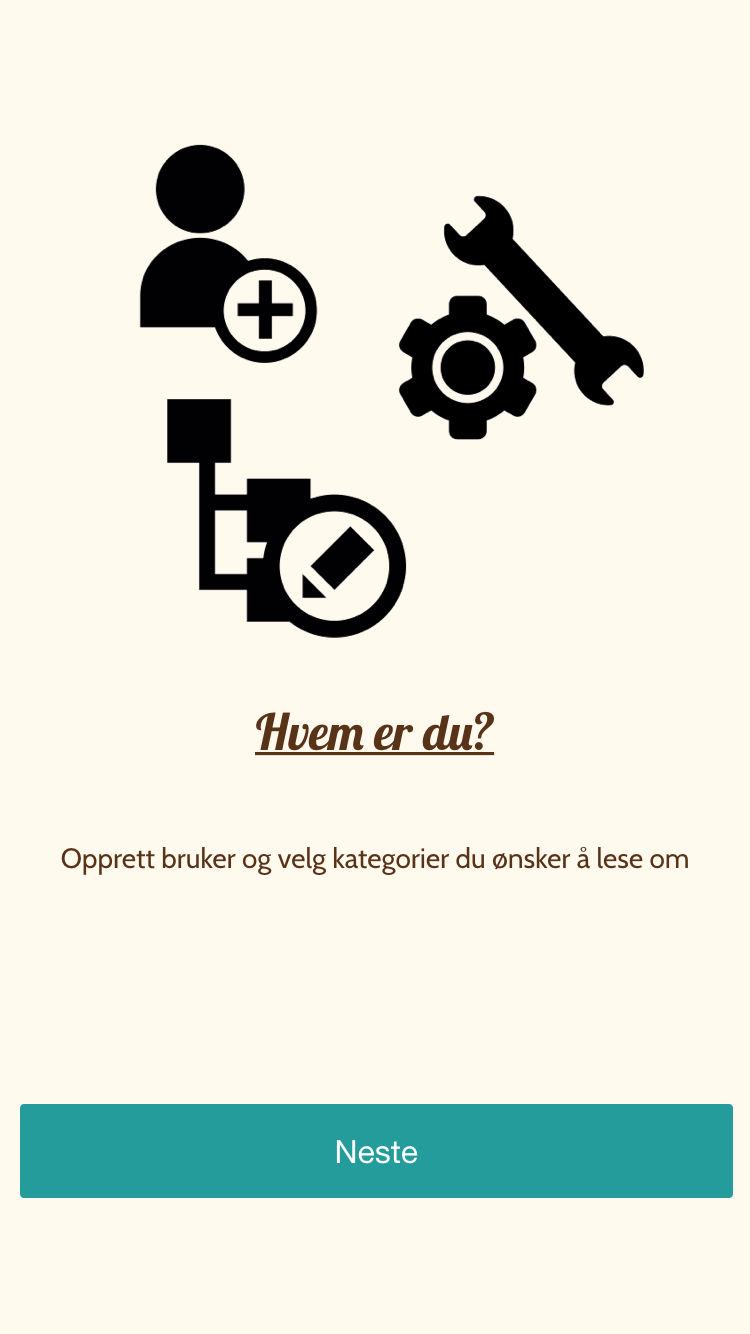
\includegraphics[width=\textwidth]{fig/screenshot_intro1}
			\caption{Introduction 1}
		\end{subfigure}
		\begin{subfigure}[h]{0.3\textwidth}
			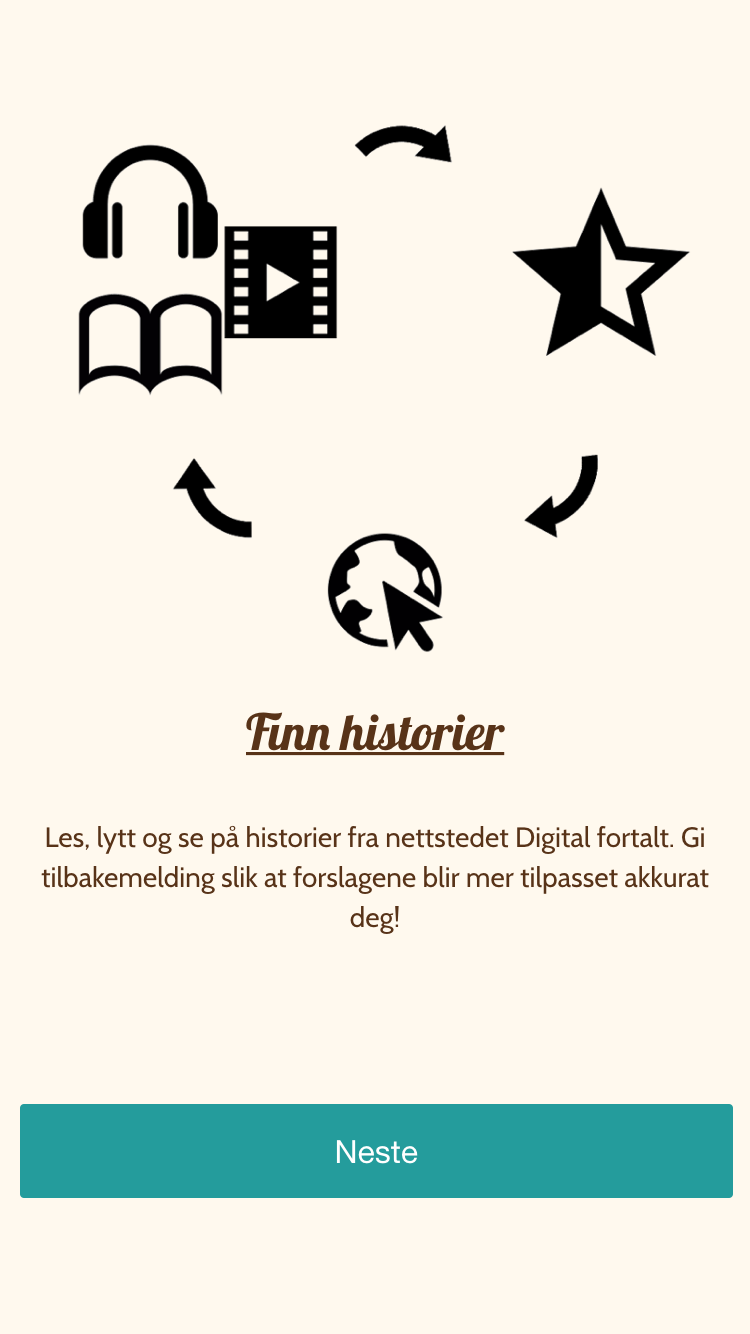
\includegraphics[width=\textwidth]{fig/screenshot_intro2}
			\caption{Introduction 2}
		\end{subfigure}
		\begin{subfigure}[h]{0.3\textwidth}
			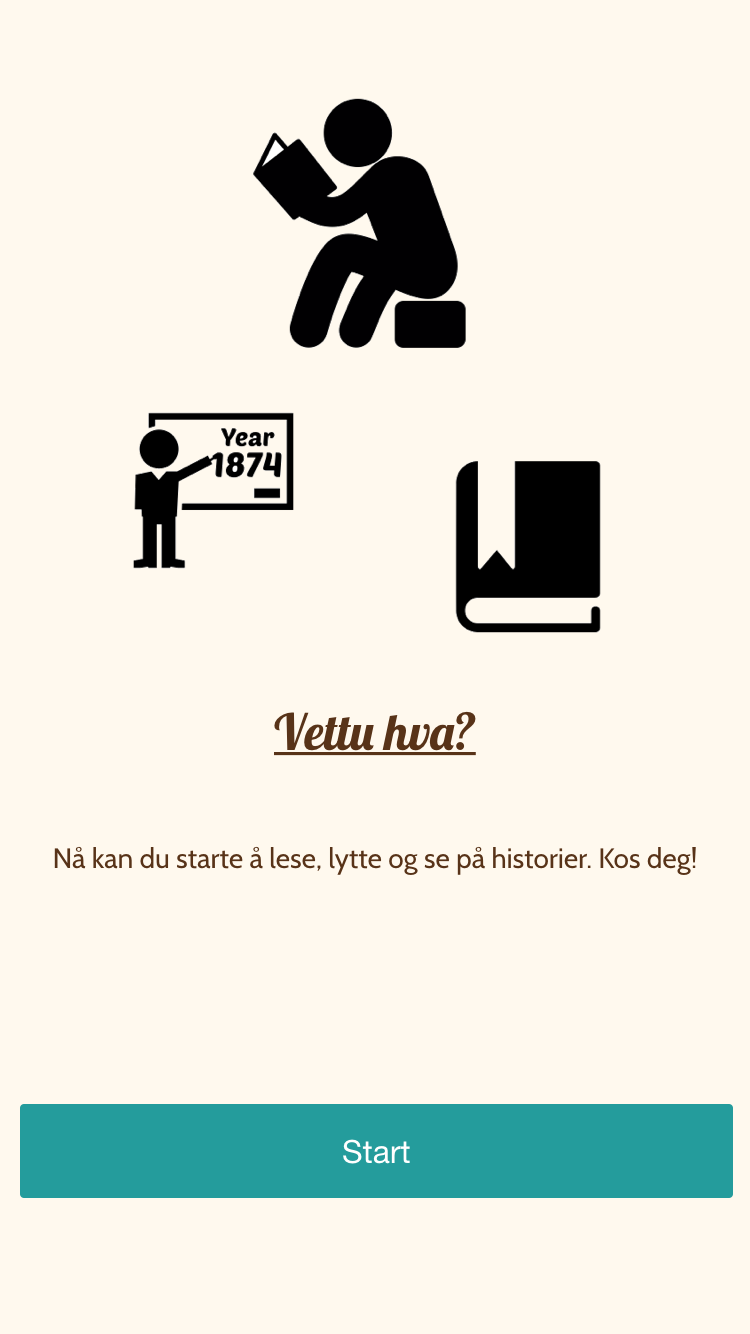
\includegraphics[width=\textwidth]{fig/screenshot_intro3}
			\caption{Introduction 3}
		\end{subfigure}

	\end{figure}
	\begin{figure}
		\ContinuedFloat
		\centering
		\begin{subfigure}[h]{0.3\textwidth}
			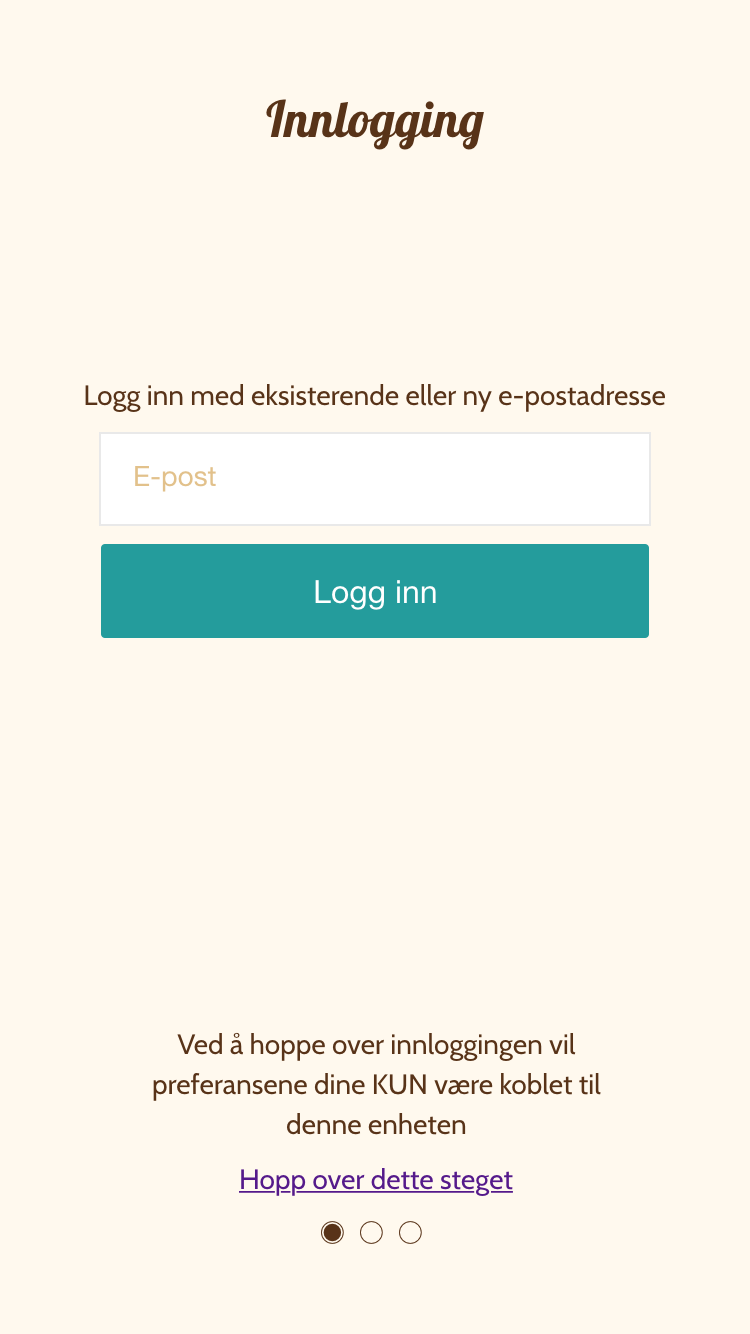
\includegraphics[width=\textwidth]{fig/screenshot_login}
			\caption{Sign in}
		\end{subfigure}
		\begin{subfigure}[h]{0.3\textwidth}
			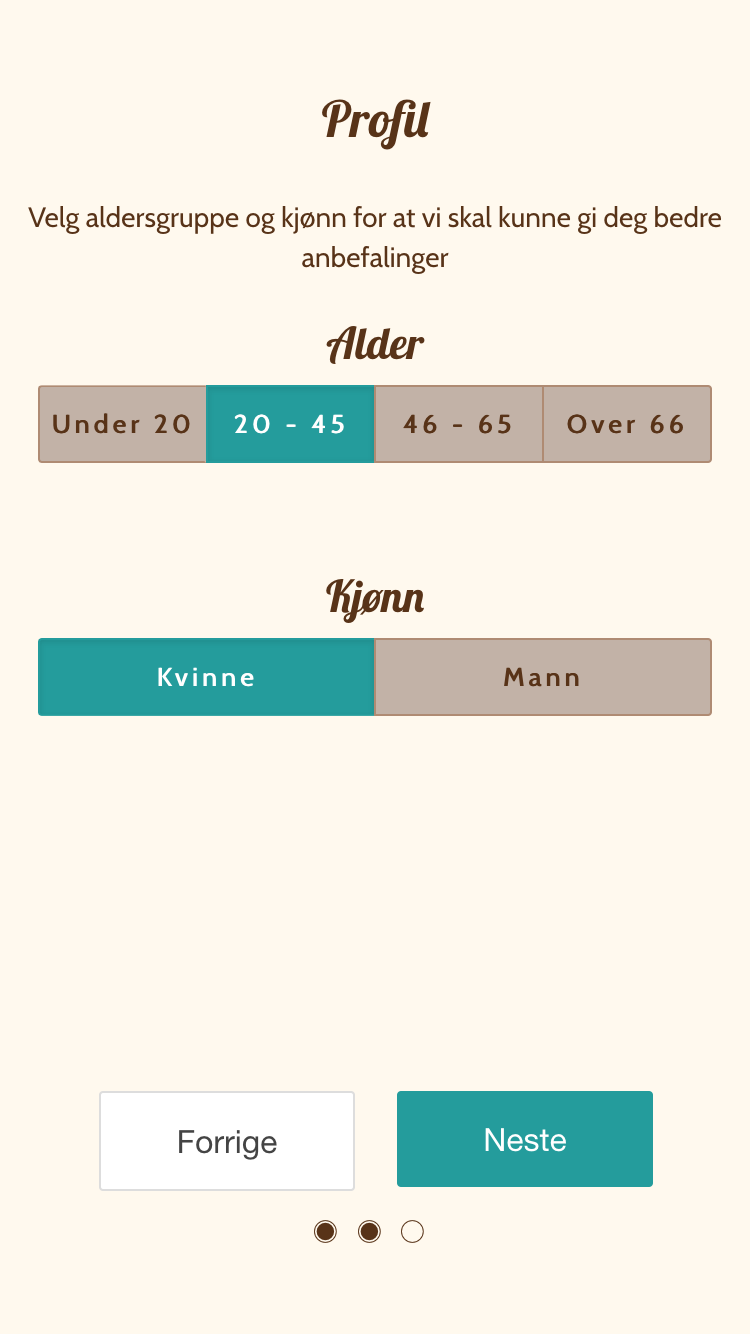
\includegraphics[width=\textwidth]{fig/screenshot_profile}
			\caption{Profile}
		\end{subfigure}
		\begin{subfigure}[h]{0.3\textwidth}
			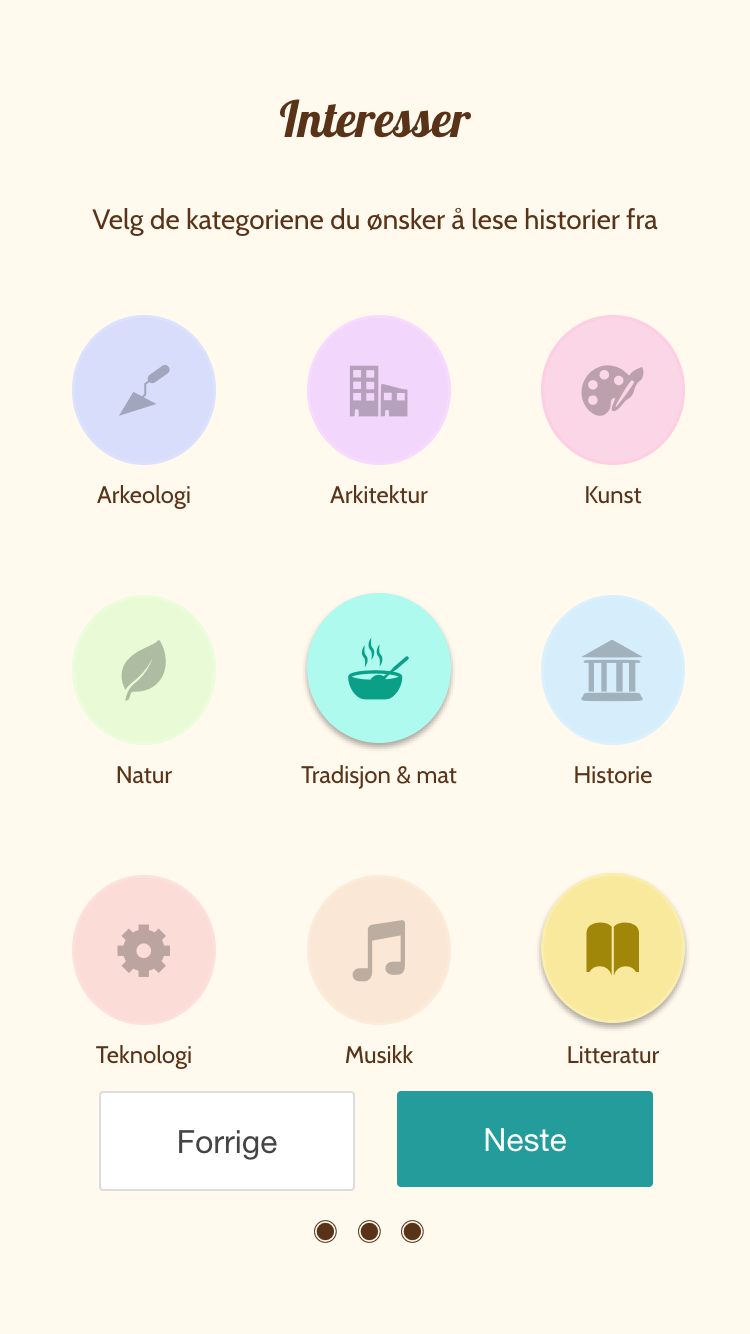
\includegraphics[width=\textwidth]{fig/screenshot_interests}
			\caption{Interests}
		\end{subfigure}
		
	\end{figure}
	\begin{figure}[h]
		\ContinuedFloat
		\centering
		\begin{subfigure}[h]{0.3\textwidth}
			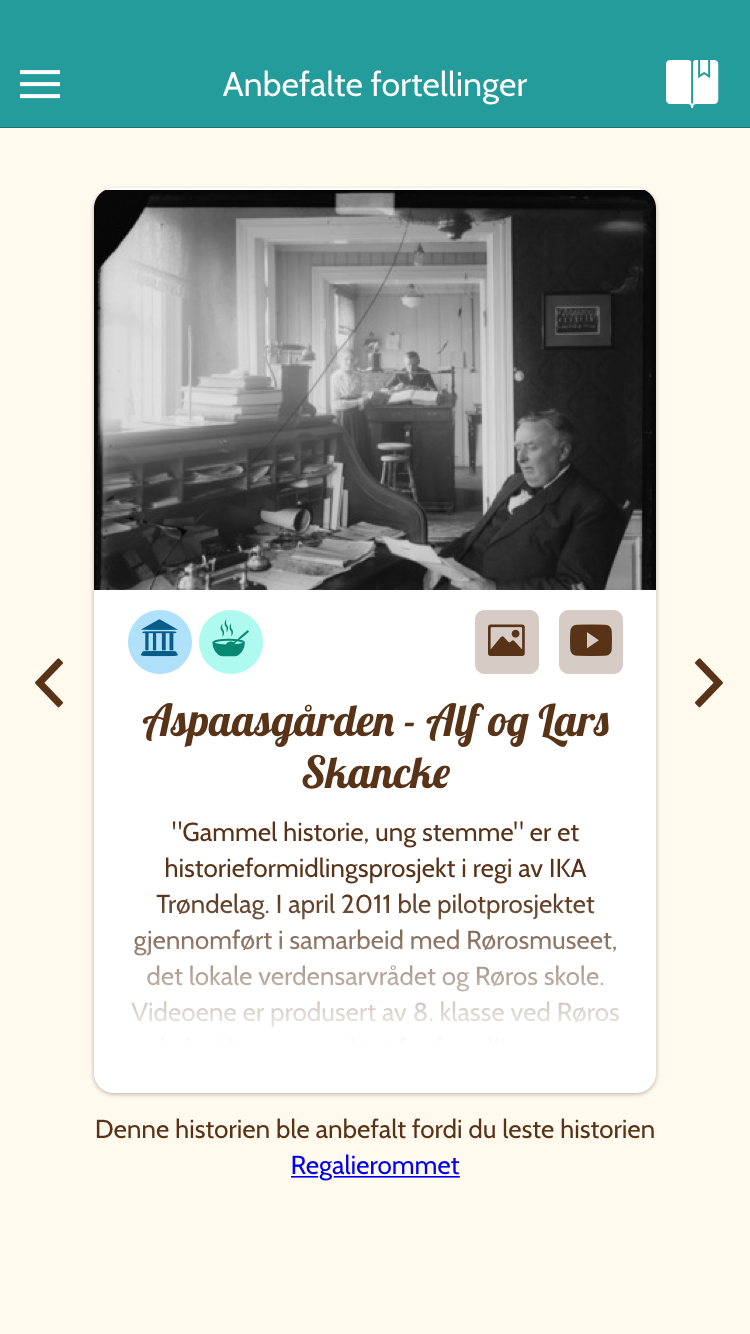
\includegraphics[width=\textwidth]{fig/screenshot_recommendations}
			\caption{Recommendations}
		\end{subfigure}
		\begin{subfigure}[h]{0.3\textwidth}
			
\includegraphics[width=\textwidth]{fig/screenshot_story}
			\caption{Story}
		\end{subfigure}
		\begin{subfigure}[h]{0.3\textwidth}
			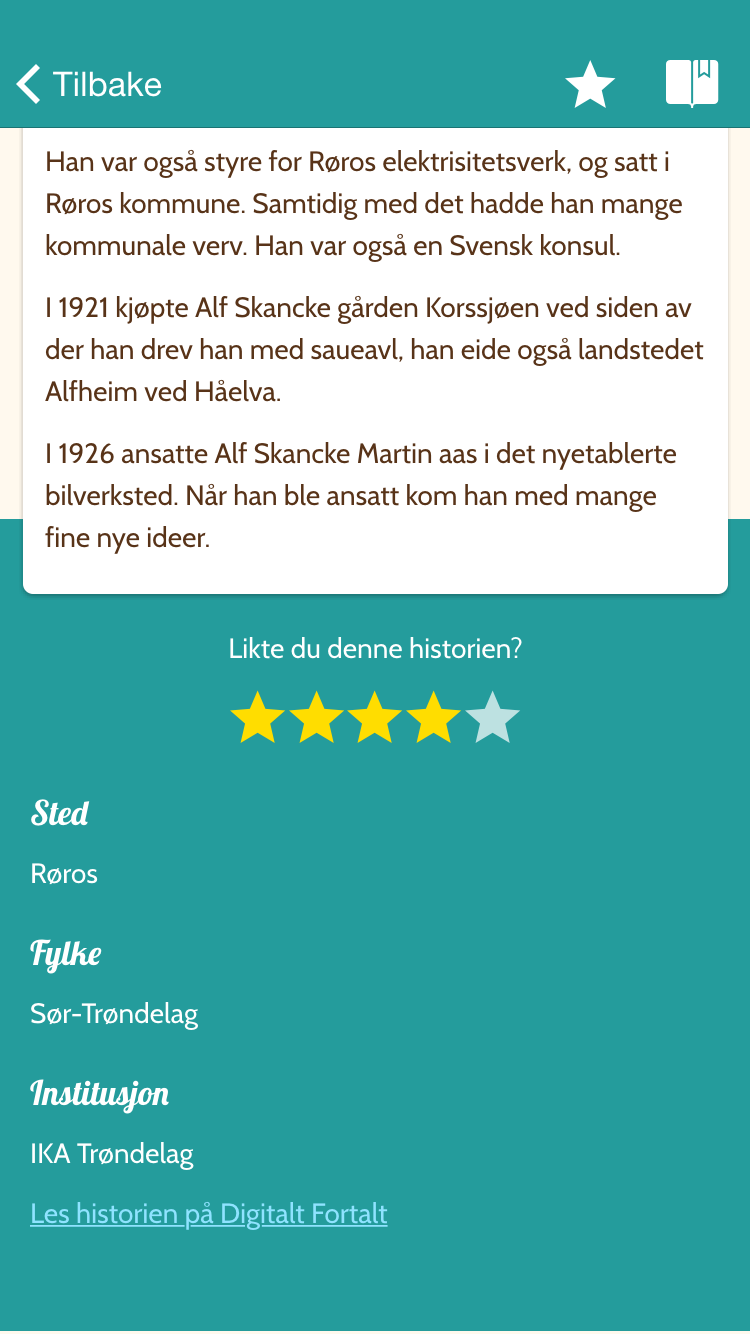
\includegraphics[width=\textwidth]{fig/screenshot_story2}
			\caption{Story 2}
		\end{subfigure}
		
	\end{figure}
	\begin{figure}[h]
		\ContinuedFloat
		\centering
		\begin{subfigure}[h]{0.3\textwidth}
			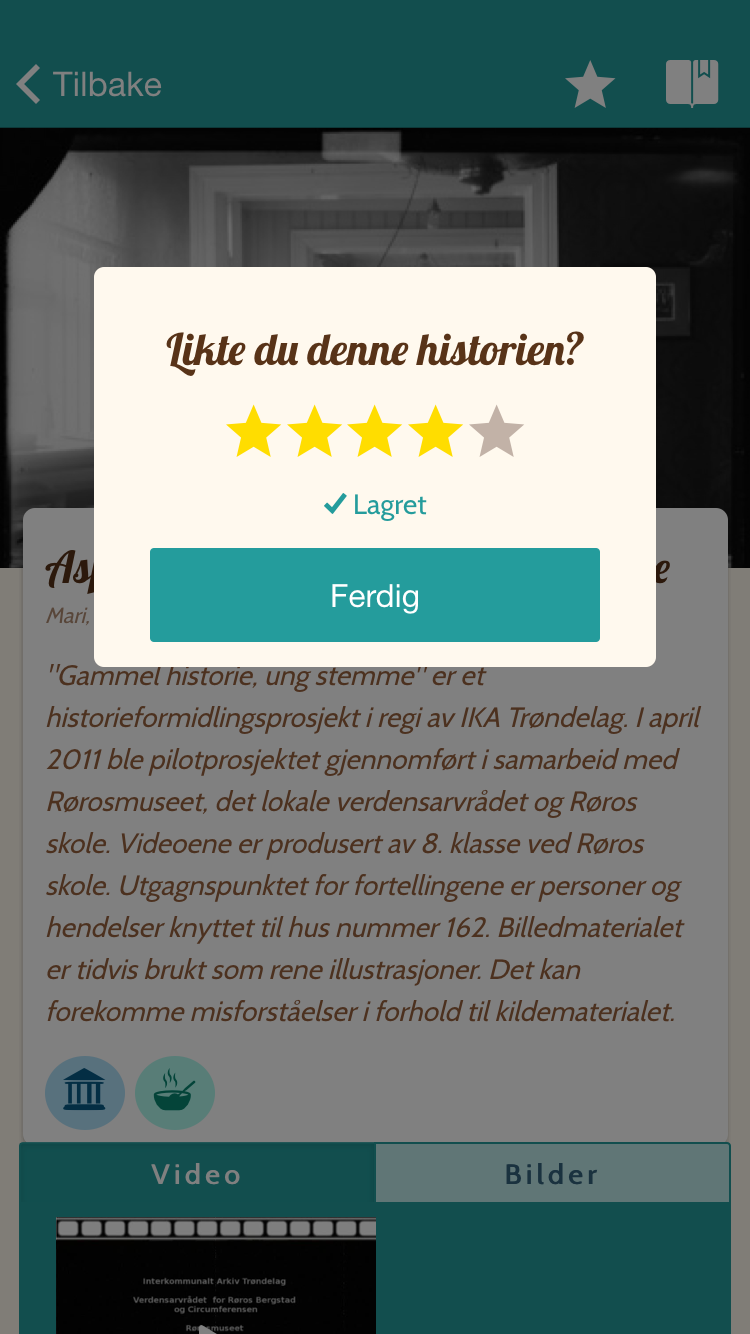
\includegraphics[width=\textwidth]{fig/screenshot_rating}
			\caption{Rating}
		\end{subfigure}
		\begin{subfigure}[h]{0.3\textwidth}
			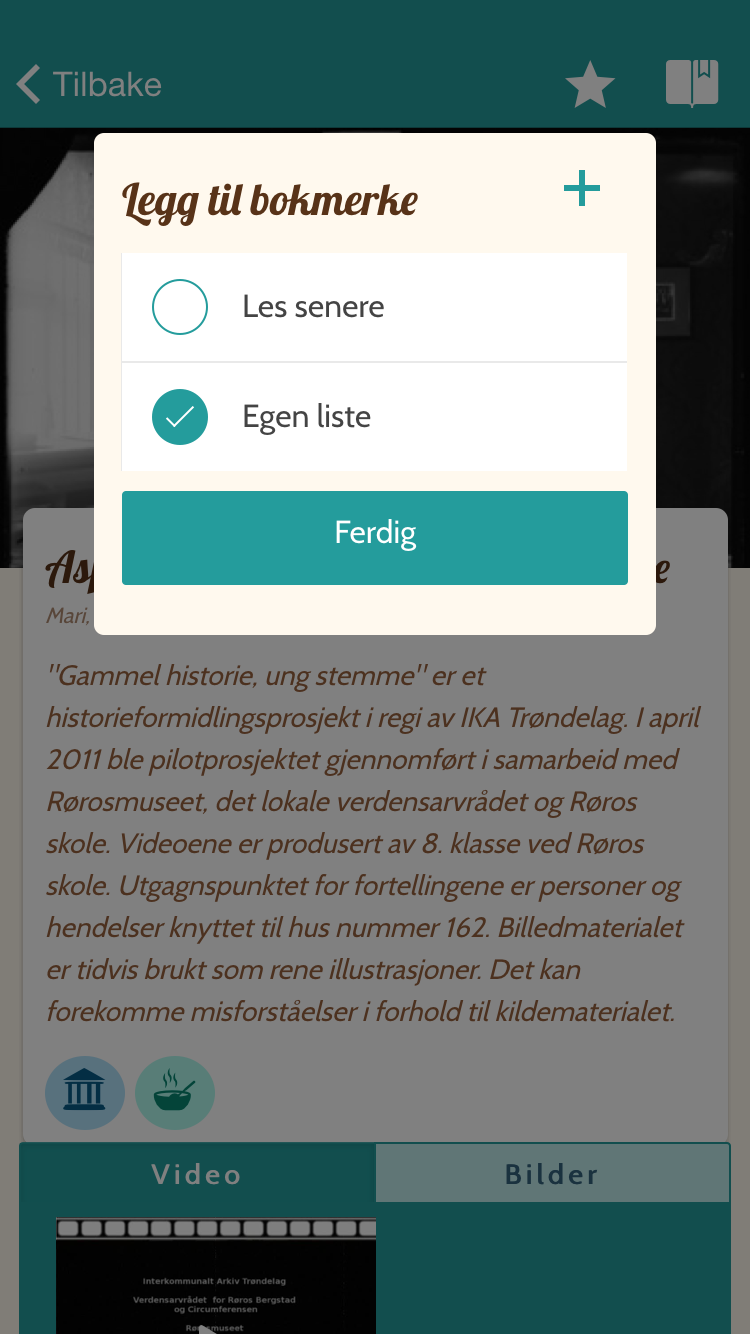
\includegraphics[width=\textwidth]{fig/screenshot_bookmark}
			\caption{Add bookmark}
		\end{subfigure}
		\begin{subfigure}[h]{0.3\textwidth}
			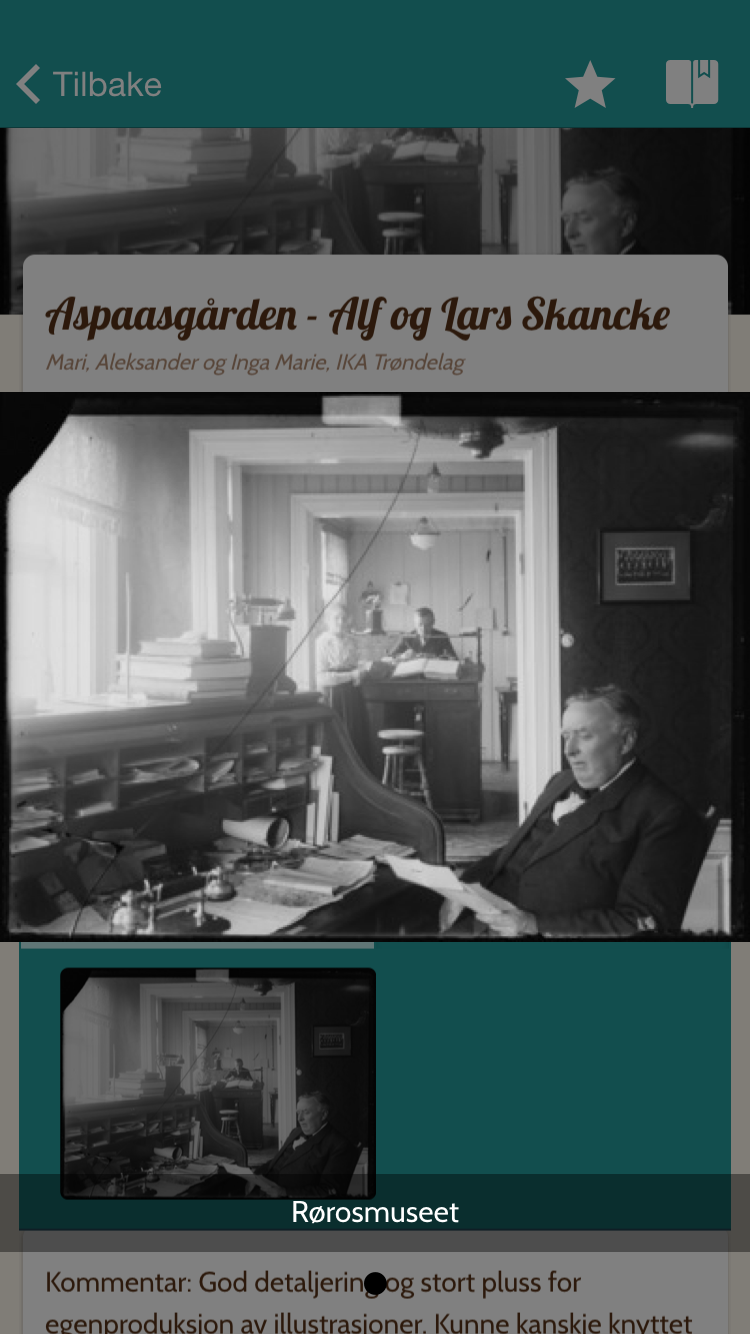
\includegraphics[width=\textwidth]{fig/screenshot_image}
			\caption{Fullscreen image}
		\end{subfigure}
	
	\end{figure}
	\begin{figure}[h]
		\ContinuedFloat
		\centering
		\begin{subfigure}[h]{0.3\textwidth}
			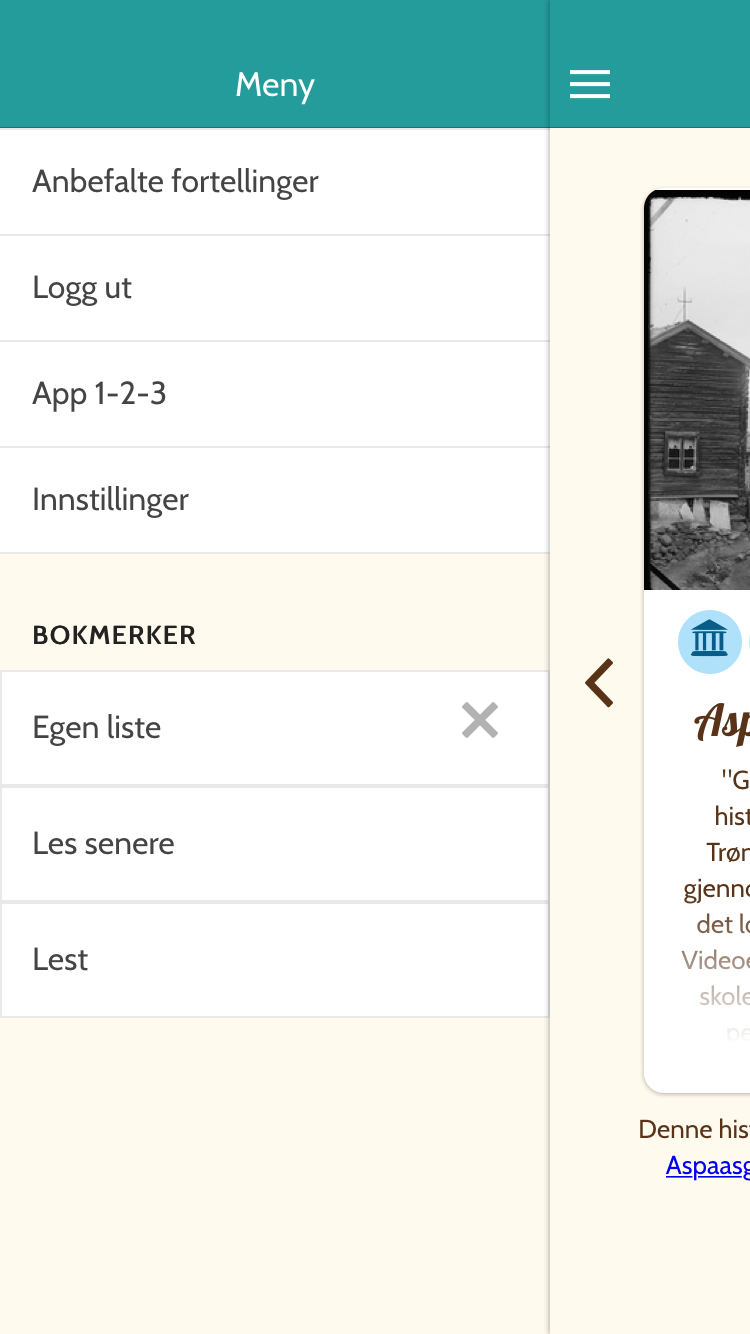
\includegraphics[width=\textwidth]{fig/screenshot_menu}
			\caption{Menu}
		\end{subfigure}
		\begin{subfigure}[h]{0.3\textwidth}
			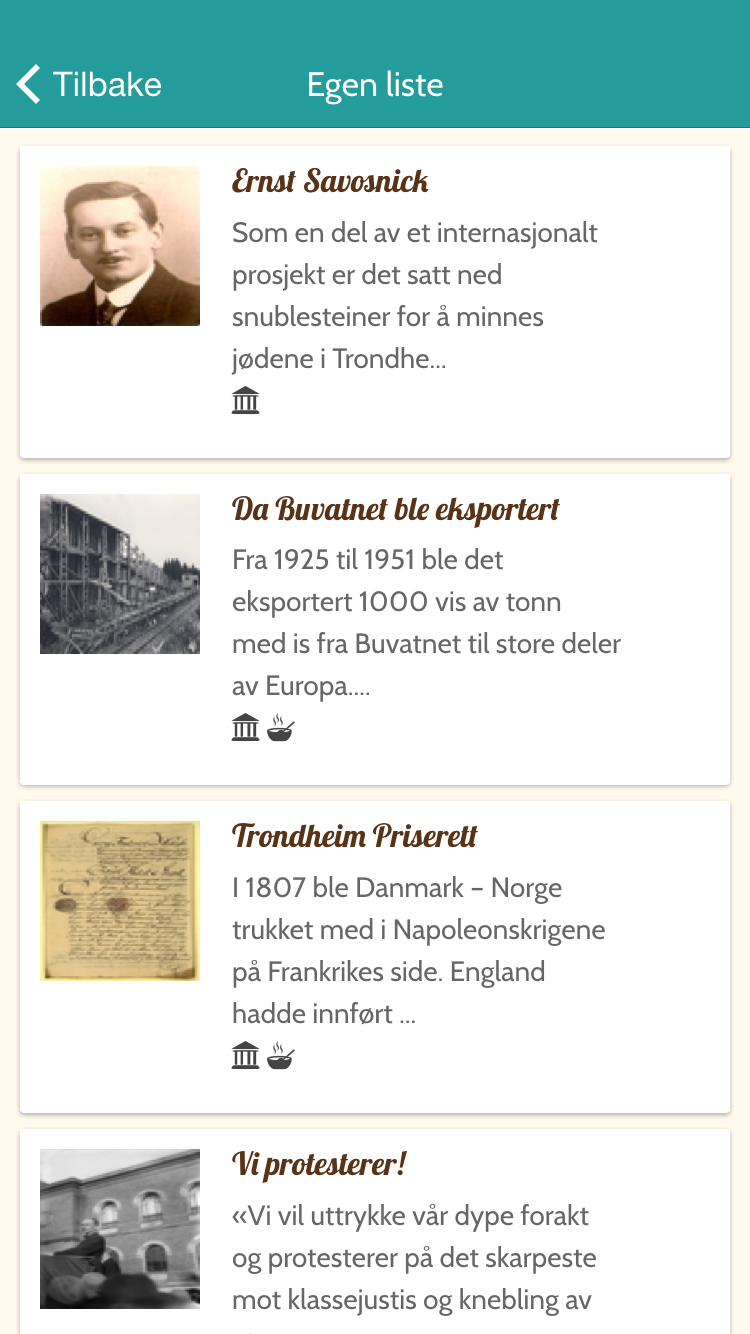
\includegraphics[width=\textwidth]{fig/screenshot_list}
			\caption{Bookmark list}
		\end{subfigure}
		\begin{subfigure}[h]{0.3\textwidth}
			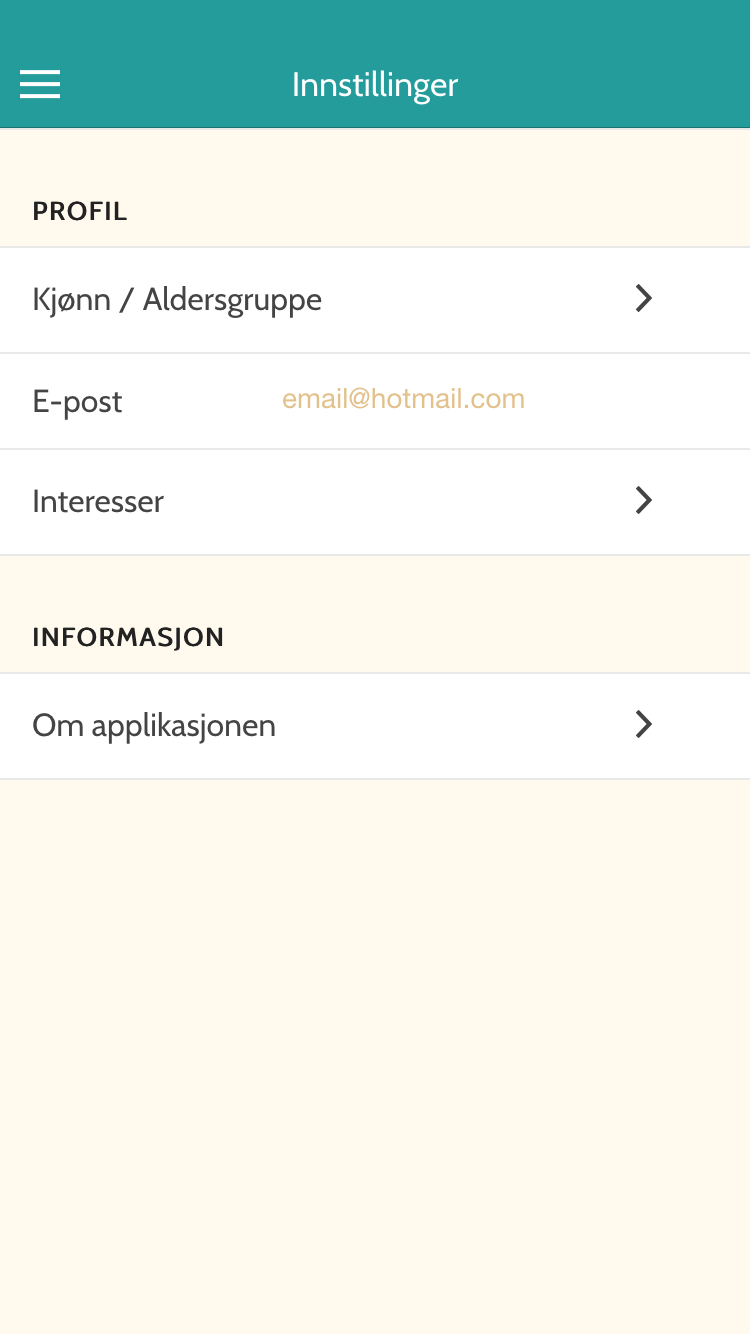
\includegraphics[width=\textwidth]{fig/screenshot_settings}
			\caption{Settings}
		\end{subfigure}
	\end{figure}

\end{appendices}
\cleardoublepage